\section{引言}

智能体强化学习（RL）已经在处理现实世界复杂问题方面展现出显著性能提升，例如 AI 编程~\citep{le2022coderl,dou2024stepcoder}、深度搜索~\citep{zheng2025deepresearcher,qi2025webrl} 与具身智能~\citep{zitkovich2023rt, wang2023voyager}。与仅依赖内部知识的传统大语言模型（LLM）不同，智能体会通过 shell 命令、API 或设备操作等外部工具主动与真实世界交互~\citep{cao2025skyrl}。为了支撑这种能力，智能体 RL 已成为后训练流程中的关键组成部分，也是云集群中的重要工作负载~\citep{xiao2026mimo}。

\begin{figure}[t]
    \centerline{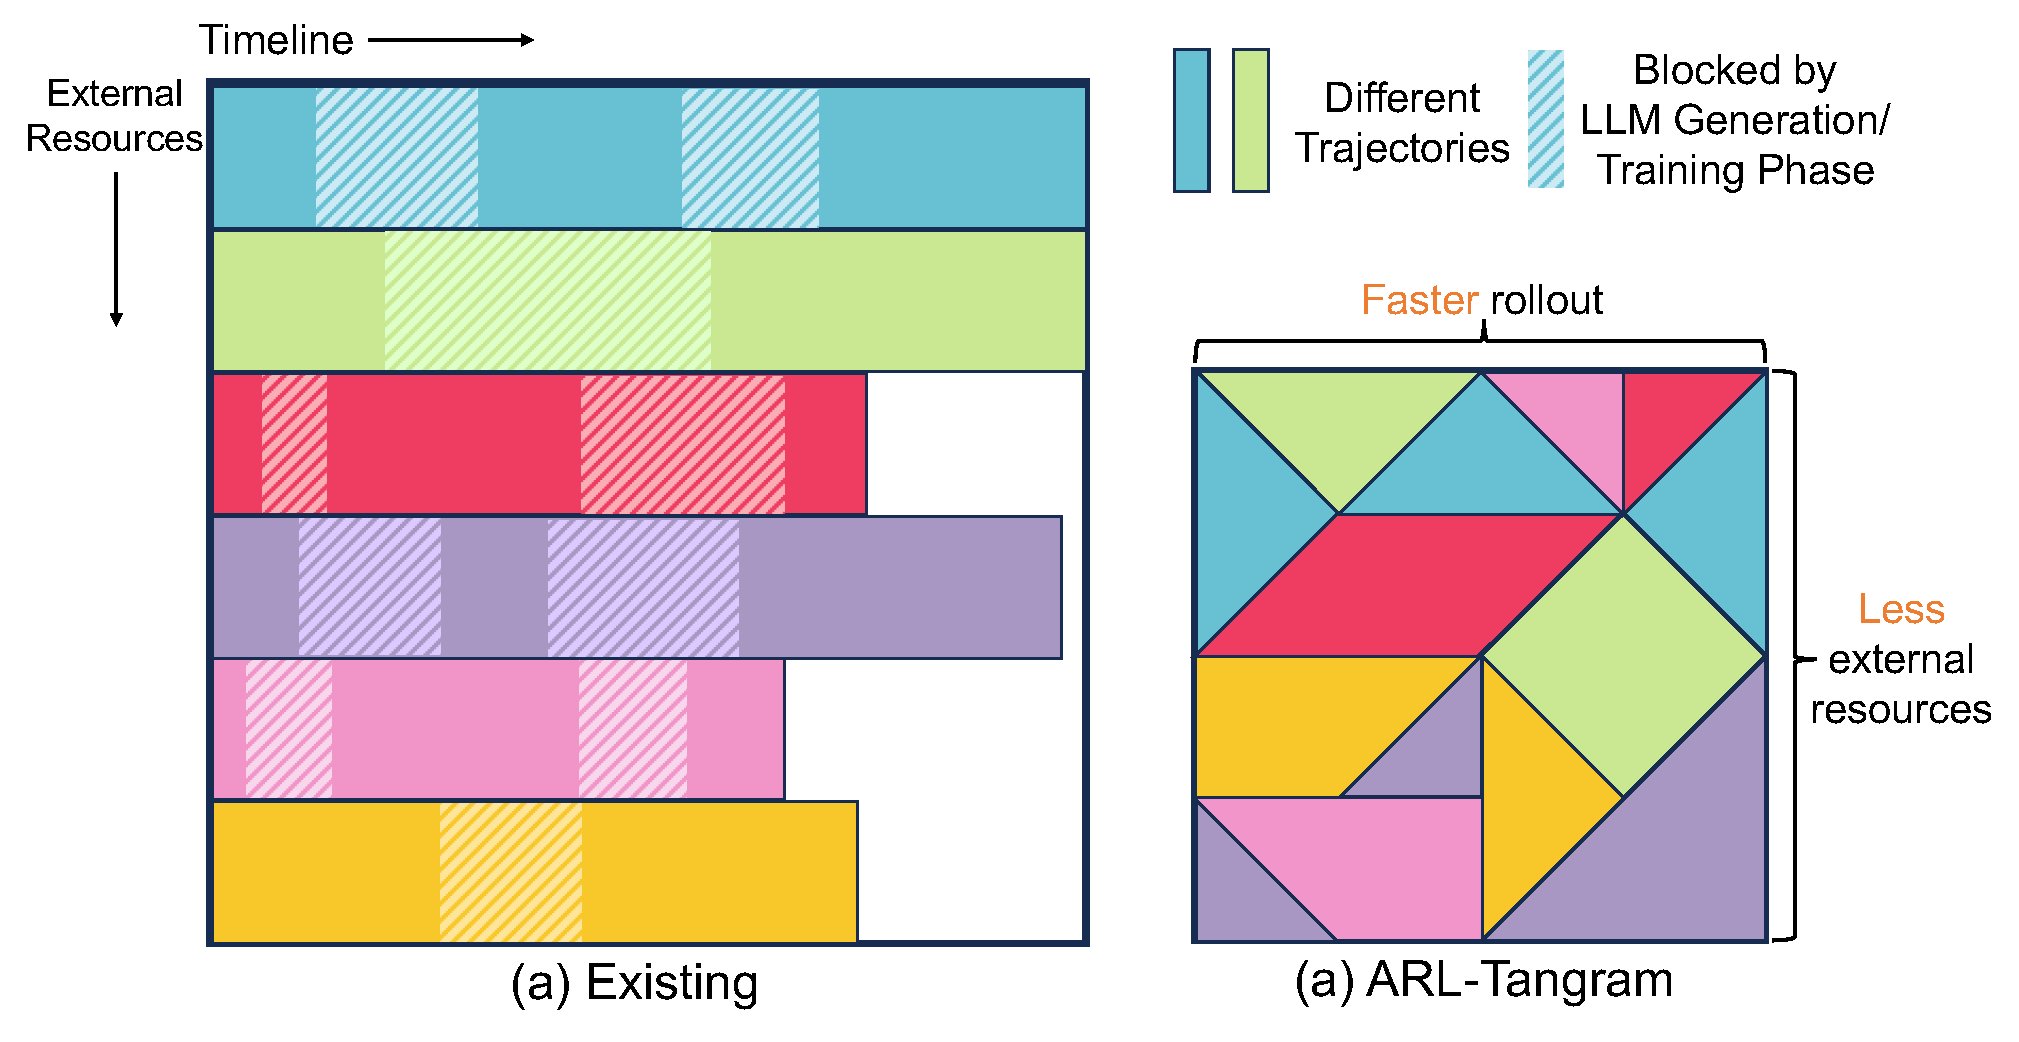
\includegraphics[width=0.9\linewidth]{figures/tangram.pdf}}
    \vspace{-0.2in}
    \caption{现有方法与 \sysname 的对比。\protect\footnotemark}
    \label{fig:intro_op}
    \vspace{-0.2in}
\end{figure}

与传统 RL 不同，智能体 RL 对外部资源有大量需求，例如 AI 编程所需的 CPU、奖励模型所需的 GPU，以及网页浏览所需的 API 配额。这些位于主训练集群之外的外部资源引入了额外的管理需求。虽然这与云资源管理问题有相似之处，但智能体场景对外部资源的高效管理提出了更高要求，主要体现在两个方面。第一，外部调用延迟与 RL 效率紧密耦合。缺乏有效的外部资源管理时，调用可能变慢甚至阻塞，不仅会拖慢训练，还可能导致整个训练流程失败。第二，外部资源带来的额外成本不容忽视。智能体 RL 的调用模式通常具有突发性，因此为了维持较低的调用延迟，往往不得不预留大量资源。所以，提高外部资源利用率并降低对应成本非常重要。

\footnotetext{该图仅用于解释 ARL-Tangram 的核心直觉，实际模式并不严格是三角形。}

然而，现有 RL 框架~\citep{sheng2025hybridflow,fu2025areal} 往往忽略了 RL 训练与外部资源使用之间的耦合关系。这些框架默认采用静态资源预留，导致外部资源出现严重浪费与低效。过量预留主要发生在两个层面（图~\ref{fig:intro_op}）。其一，在轨迹层面，系统通常会在一条轨迹的整个生命周期中长期保留专用资源，即便这些资源只在少数时刻被调用。例如在 AI 编程中，环境平均仅有 47\% 的生命周期真正被访问，剩余时间所占用的 CPU 都被浪费了。其二，在 RL 任务层面，不同任务通常需要特定的外部服务，这些服务会部署在相互隔离的资源上~\citep{jiang2025verltool,micromulti}。但由于外部调用模式波动很大，这些资源长期处于低利用率状态。总之，这种静态管理限制了系统并发度，增加了调用排队延迟，并拖慢了 RL 训练。

为了解决这些问题，我们提出 \textbf{动作级} 调度，把外部资源管理粒度从原先的轨迹级或任务级下沉到更细的动作级，即原子调用的粒度。我们把寿命较长的环境或服务占用拆解为动作级占用，并把相同资源类型对应的资源统一池化给动作使用。除此之外，这种细粒度管理还允许系统进行弹性资源分配，从而降低动作执行延迟。正如图~\ref{fig:intro_op} 所示，当有两个 RL 任务、四条轨迹访问同类外部资源时，动作级调度相比现有方法可以通过缓解过量预留来减少所需外部资源，并通过弹性分配来加速 rollout。

不过，实现动作级调度并不简单，主要有三个原因。第一，面向多种外部资源对动作进行统一编排本身就很复杂。单个动作可能同时依赖多种资源类型，而不同动作的弹性与执行模式又各不相同，因此需要一个通用抽象模型。第二，调度器必须面对强延迟敏感工作负载。动作持续时间可能只有微秒级，这意味着调度决策窗口极短，需要足够轻量的算法来处理高并发和突发流量。第三，如何统一且高效地管理具有不同特征与拓扑结构的异构外部资源同样具有挑战。

因此，我们设计了 \sysname（\textbf{A}gentic \textbf{R}einforcement \textbf{L}earning \textbf{Tangram}），一个动作级资源管理系统，用来统一编排这些外部资源调用。首先，它采用统一的动作建模来描述具有异构资源需求和成本的动作。系统把每个动作表示为向量化的资源成本，其中包含 CPU、GPU、内存以及 API 配额等多种约束。更关键的是，这一建模还纳入了弹性刻画，使系统能够识别弹性动作，并计算在分配更多资源时动作时延如何下降。借助这一建模，\sysname 能把不同类型的动作归一化成统一格式供调度器处理。

\sysname 的核心是一个面向最小化动作完成时间（ACT）的弹性资源调度算法。考虑到更短的动作执行时间会直接提升端到端智能体 RL 训练效率，我们提出了一个带贪心驱逐机制的启发式调度算法，它根据统一建模与实时系统状态来编排动作。这个贪心驱逐策略会动态确定资源分配方式，从而避免过于激进或过于保守的分配导致次优 ACT 和较差的 RL 效率。

在调度器之外，\sysname 还为异构资源设计了专门的资源管理器。每类管理器都提供相应机制，用于高效地实现 \textbf{Breakdown}，也就是在每个动作执行后释放资源，同时保留环境或服务状态并在再次调用时快速恢复；以及 \textbf{Pool}，也就是在缓解碎片化并提升并行效率的原则下进行资源分配。尽管资源在特征和拓扑上高度异构，这些管理器仍通过统一接口向调度器暴露能力，从而让调度算法对底层异构性保持透明。

我们将 \sysname 实现为一个独立于 RL 框架、外部调用类型和外部资源类型的系统。这一设计带来了更强的通用性与更低的接入复杂度。我们在真实世界智能体 RL 训练任务上评估 \sysname，结果表明它可将平均 ACT 最多降低 4.3$\times$，把 RL 训练 step 时长最多加速 1.5$\times$，并最多节省 71.2$\%$ 的外部资源。该系统已被用于支持 MiMo 系列模型的 RL 训练。

总的来说，本文贡献如下：
\begin{itemize}[leftmargin=10pt]
    \item 我们分析了智能体 RL 训练中外部资源过量预留这一关键问题，并把它归纳为轨迹内过量预留和 RL 任务内过量预留两类。
    \item 我们提出动作级调度，并将其实现为统一资源管理系统 \sysname，把管理粒度从轨迹级下沉到动作级，从而实现细粒度共享与弹性调度。
    \item 我们设计了统一的动作建模以及面向最小化 ACT 的弹性调度算法，并结合异构资源专用管理器进一步提升外部资源利用率与训练效率。
    \item 我们在真实 RL 训练任务上评估 \sysname，证明它能够显著提升智能体 RL 的端到端效率，并降低外部资源成本。
\end{itemize}
